\documentclass{../../ece-report}

\memostudent{Ty Davis}
\memotitle{Lab 2 - Rectifier Circuits}
\memocourse{ECE 3110}
\memodate{\today}

\newcommand{\ra}[1]{\renewcommand{\arraystretch}{#1}}

\begin{document}
\maketitle
\section{Introduction}

In this lab we are analyzing the performance of three
different rectifier circuits, namely a half-wave rectifier,
a peak rectifier, and a precision rectifier. For each
circuit shown we will simulate the circuit, then build
and measure what we simulated to compare.

This lab is going to have a lot of figures and tables.

\section{Half-wave Rectifier}

The half-wave rectifier, as shown in Fig.~\ref{fig:half_wave_circuit},
is a circuit that cuts out the negative portion of an
AC wave. With an ideal diode, we would be able to get
a perfect positive-portion of an AC wave without any
power loss, but because the diodes show a voltage drop
when forward-biased, the output is always a touch lower
than the input. Refer to Fig.~\ref{fig:half_wave_plots}
to see the slight decrease on the output. Measured values
are shown in Table~\ref{tab:half_wave}.

\begin{figure}[h!]
  \centering
  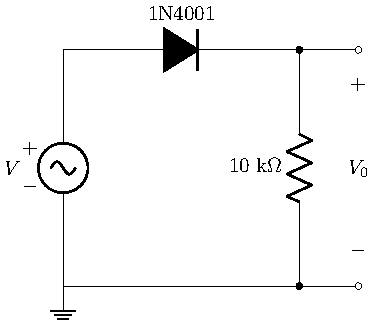
\includegraphics{../circuits/half_wave_circuit.pdf}
  \caption{Half-wave Rectifier Circuit}
  \label{fig:half_wave_circuit}
\end{figure}


\begin{table}[h!]
  \centering
  \begin{tabular}{rrrrcrrr}\toprule
    & \multicolumn{3}{c}{$10~\si{\V}_\textnormal{pp}$} & & \multicolumn{3}{c}{$0.5~\si{\V}_\textnormal{pp}$} \\
    \cmidrule(lr){2-4} \cmidrule(lr){6-8}
    & Simulated & Simulated 9.74~\si{\kohm} & Measured & & Simulated & Simulated 9.74~\si{\kohm} & Measured \\
    V$_\textnormal{MAX}$ & 4.503  & 4.502  & 4.502  & & 0.025  & 0.024  &  0.003 \\
    V$_\textnormal{MIN}$ & -0.011 & -0.010 & -0.080 & & -0.001 & -0.001 & -0.001 \\
    V$_\textnormal{pp}$ &  4.513  & 4.612  & 4.583  & & 0.025  & 0.025  & -0.004 \\
    \bottomrule
  \end{tabular}
  \caption{Half Wave Rectifier Simulation and Measurement Values}
  \label{tab:half_wave}
\end{table}

\begin{figure}[h!]
  \centering
  \begin{minipage}{.45\textwidth}
    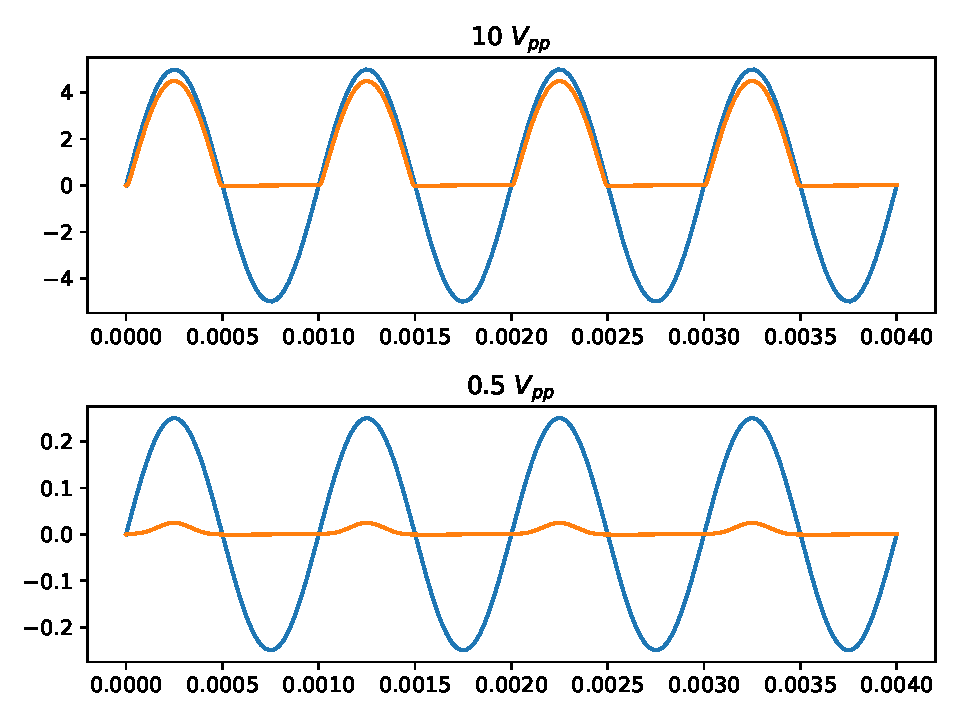
\includegraphics[width=\textwidth]{../figures/half-wave/half-wave-sim.pdf}
  \end{minipage}
  \begin{minipage}{.45\textwidth}
    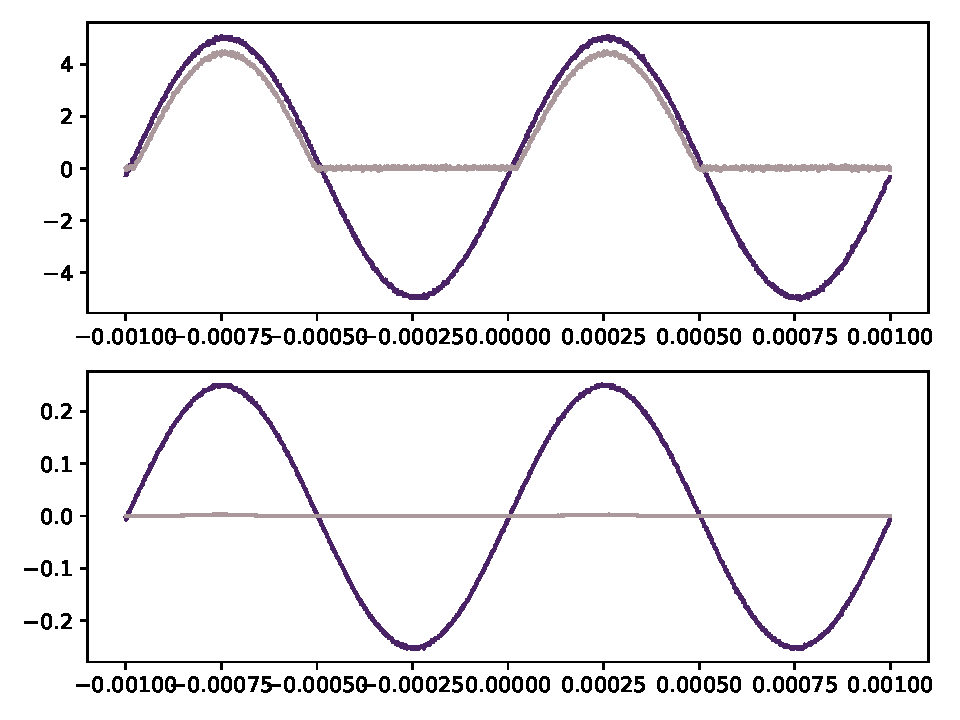
\includegraphics[width=\textwidth]{../figures/half-wave/half-wave-measured.pdf}
  \end{minipage}
  \caption{Half-wave Rectifier Circuit Plots}
  \label{fig:half_wave_plots}
\end{figure}

\section{Peak Rectifier}

The peak rectifier is very similar to the half-wave
rectifier, but it utilizes a capacitor in parallel with
the output to maintain a high voltage on the output.
This effectively converts an AC signal to DC, and can
be clearly seen in Fig.~\ref{fig:peak_plots}. Measured
values are captured in Table~\ref{tab:peak}.

Choosing an appropriate resistor to show the output
is important if the electronics connected to the output
are sensitive to small changes in DC power. The output
shows a small ripple voltage (which can also be seen
in Table~\ref{tab:peak}). If the goal is to keep a small
ripple voltage, the correct capacitor/resistor combination
will be desired to keep the decay to a minimum during
the negative portion of the input sine wave.

\begin{figure}[h!]
  \centering
  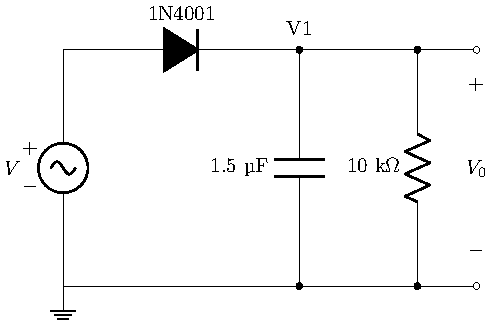
\includegraphics{../circuits/peak_circuit.pdf}
  \caption{Peak Rectifier Circuit}
  \label{fig:peak_circuit}
\end{figure}

\begin{table}[h!]
  \centering
  \begin{tabular}{rrrrcrrr}\toprule
    & \multicolumn{3}{c}{$47~\si{\kohm}$} & & \multicolumn{3}{c}{$4.7~\si{\kohm}$} \\
    \cmidrule(lr){2-4} \cmidrule(lr){6-8}
    & Simulated & Simulated 44.8~\si{\kohm} & Measured & & Simulated & Simulated 4.607~\si{\kohm} & Measured \\
    V$_\textnormal{MAX}$ & 4.453 & 4.452  & 4.342  & & 4.419  & 4.418  & 4.020 \\
    V$_\textnormal{MIN}$ & 4.392 & 4.388  & 4.020  & & 3.898  & 3.888  & 3.377 \\
    Ripple               & 0.025 & 0.063  & 0.322  & & 0.521  & 0.531  & 0.643 \\
    \bottomrule
  \end{tabular}
  \caption{Peak Rectifier Simulation and Measurement Values}
  \label{tab:peak}
\end{table}

\begin{figure}[h!]
  \centering
  \begin{minipage}{.45\textwidth}
    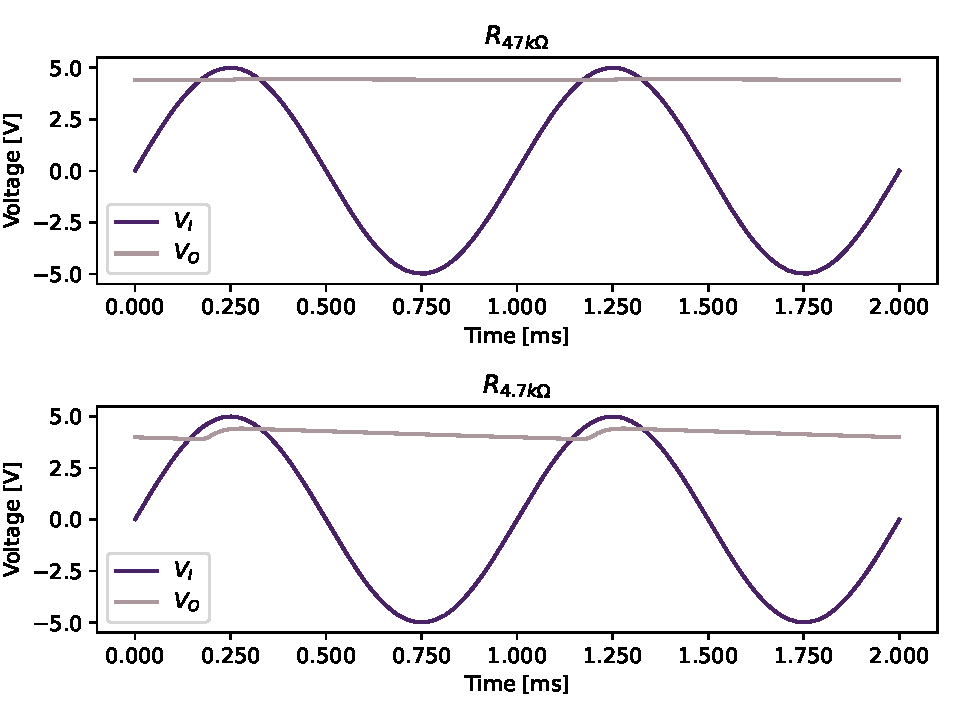
\includegraphics[width=\textwidth]{../figures/peak/peak_sim.pdf}
  \end{minipage}
  \begin{minipage}{.45\textwidth}
    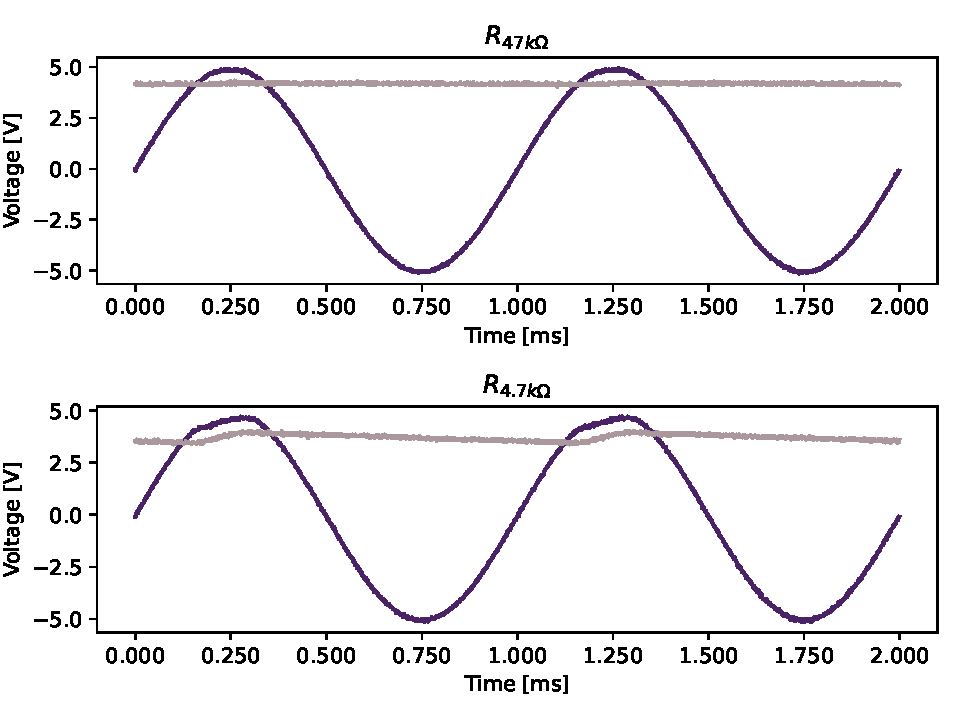
\includegraphics[width=\textwidth]{../figures/peak/peak_measured.pdf}
  \end{minipage}
  \caption{Peak Rectifier Circuit Plots}
  \label{fig:peak_plots}
\end{figure}

\section{Precision Rectifier}

The precision rectifier is a circuit which utilizes
an op amp to effectively operate like an ideal diode
and remove the voltage drop on the positive side that
occurred with the half-wave rectifier circuit. The result
is an almost perfect half-sine, but when the voltage is near
zero there is some distortion. It is even more prevalent
when the amplitude of the input voltage is low. This is seen
if Fig.~\ref{fig:precision_plots}, and the values from the 
measurements and simulation are shown in Table~\ref{tab:precision}.

\begin{figure}[h!]
  \centering
  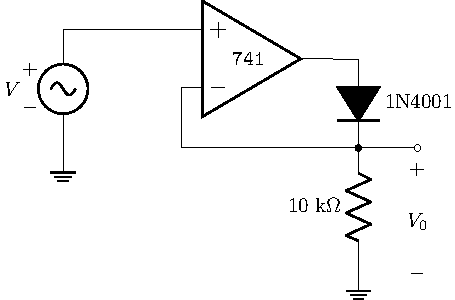
\includegraphics{../circuits/precision_circuit.pdf}
  \caption{Precision Rectifier Circuit}
  \label{fig:precision_circuit}
\end{figure}

\begin{table}[h!]
  \centering
  \begin{tabular}{rrrrcrrr}\toprule
    & \multicolumn{3}{c}{$10~\si{\V}_\textnormal{pp}$} & & \multicolumn{3}{c}{$0.5~\si{\V}_\textnormal{pp}$} \\
    \cmidrule(lr){2-4} \cmidrule(lr){6-8}
    & Simulated & Simulated 9.74~\si{\kohm} & Measured & & Simulated & Simulated 9.74~\si{\kohm} & Measured \\
    V$_\textnormal{MAX}$ & 4.991  & 4.993  & 5.025  &    & 0.250  & 0.250  & 0.249  \\
    V$_\textnormal{MIN}$ & -0.010 & -0.010 & -0.352 &    & -0.032 & -0.031 & -0.024 \\
    V$_\textnormal{pp}$ &  5.091  & 5.090  & 5.377  &    & 0.282  & 0.281  & 0.273 \\
    \bottomrule
  \end{tabular}
  \caption{Precision Rectifier Simulation and Measurement Values}
  \label{tab:precision}
\end{table}

\begin{figure}[h!]
  \centering
  \begin{minipage}{.45\textwidth}
    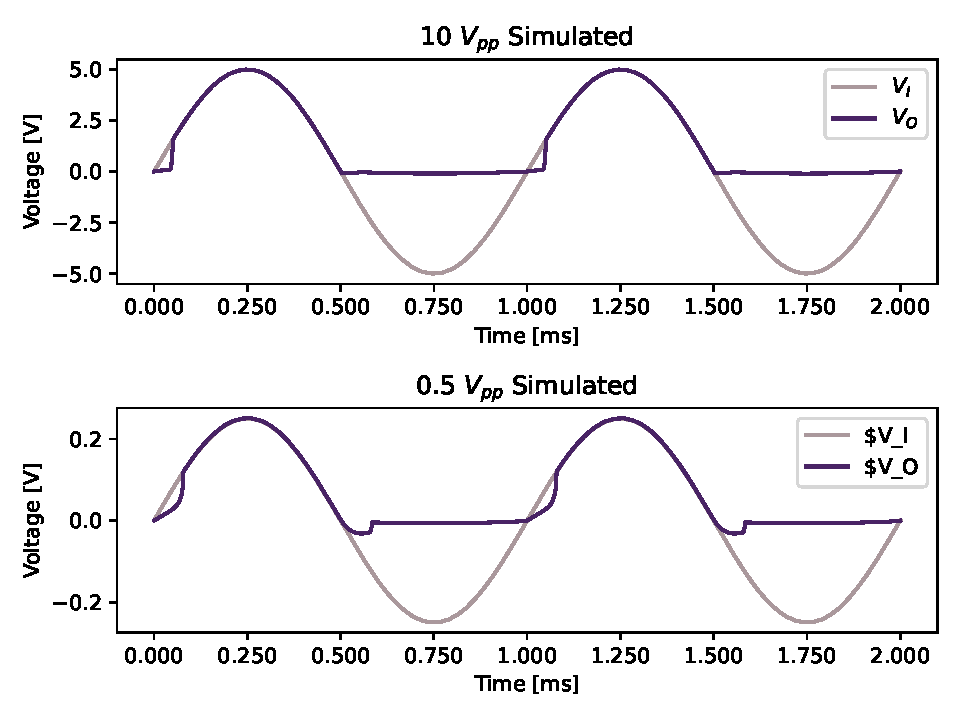
\includegraphics[width=\textwidth]{../figures/precision/precision_sim.pdf}
  \end{minipage}
  \begin{minipage}{.45\textwidth}
    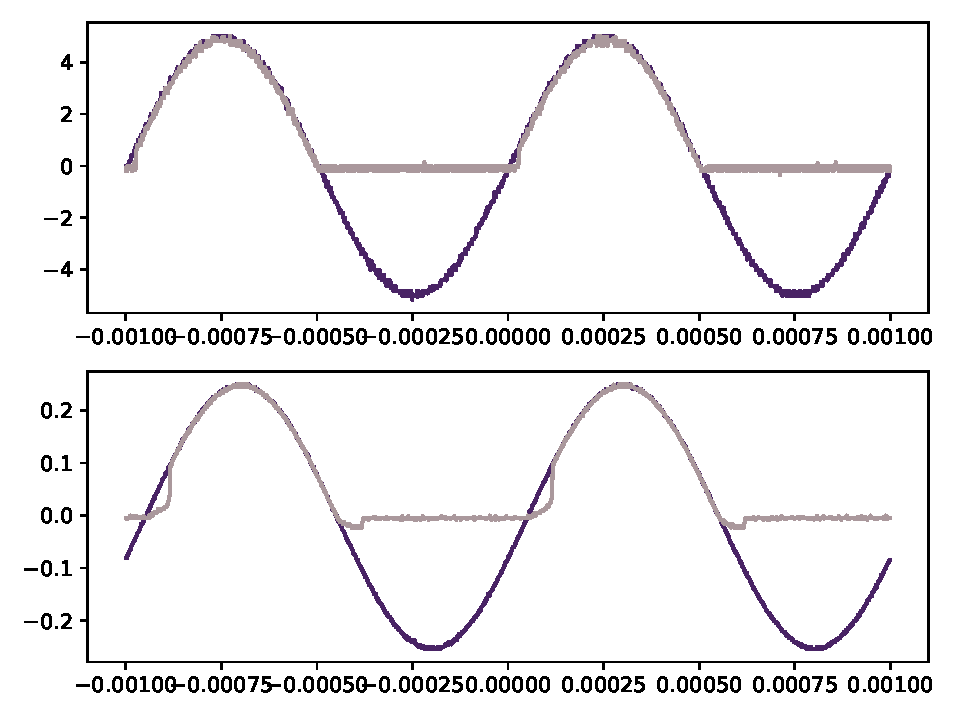
\includegraphics[width=\textwidth]{../figures/precision/precision_measured.pdf}
  \end{minipage}
  \caption{Precision Rectifier Circuit Plots}
  \label{fig:precision_plots}
\end{figure}

\section{Conclusion}

Our simulations of the rectifier circuits were very
similar to the measured outputs that we captured when
we built the circuit. I thought the most interesting
circuit that we analyzed was the precision rectifier,
I wasn't expecting so much distortion on the output.
It seemed that the distortion occurred when the diode
was no longer forward biased. I wonder if an ideal diode
would be the solution to making this a perfect half-sine
as well.

I also thought it was interesting that the voltage of
the input was affected by the peak rectifier circuit when
it was measured. I wasn't able to find a logical conclusion
for why that occurred when we were just directly measuring
the input from the function generator.

\end{document}
